\chapter{需求建模 }
\section{数据流图}
\subsection{顶层数据流图}
%top_level_DFD.png
\begin{figure}[ht]
	\centering
	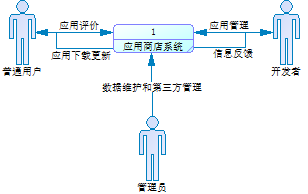
\includegraphics[width=7cm]{top_level_DFD.png}
	\caption{顶层数据流图} \label{fig:top_level_DFD}
\end{figure}
见图\ref{fig:top_level_DFD}

\subsection{0层数据流图}
\begin{figure}[ht]
	\centering
	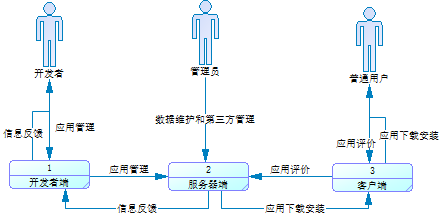
\includegraphics[width=10cm]{0_level_DFD.png}
	\caption{0层数据流图} \label{fig:0_level_DFD}
\end{figure}
见图\ref{fig:0_level_DFD}

\subsection{1层数据流图}
\begin{figure}[ht]
	\centering
	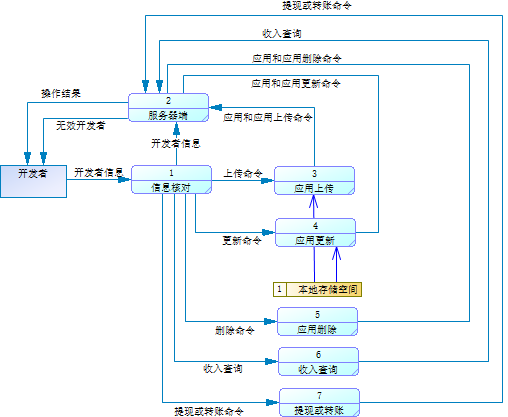
\includegraphics[width=12cm]{1_level_DFD_developer.png}
	\caption{1层数据流图-开发者端} \label{fig:1_level_DFD_dveloper}
\end{figure}
开发者端的1层数据流图见图\ref{fig:1_level_DFD_dveloper}

\begin{figure}[ht]
	\centering
	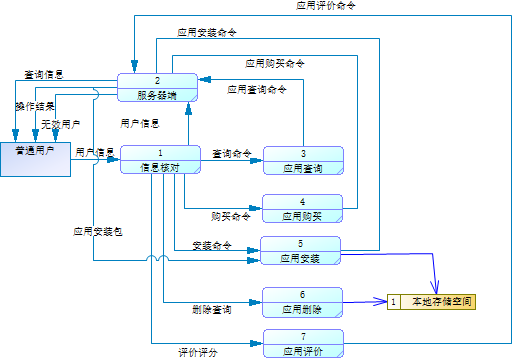
\includegraphics[width=12cm]{1_level_DFD_client.png}
	\caption{1层数据流图-客户端} \label{fig:1_level_DFD_client}
\end{figure}

客户端的1层数据流图见图\ref{fig:1_level_DFD_client}


%1_level_DFD_server.png
\begin{figure}[ht]
	\centering
	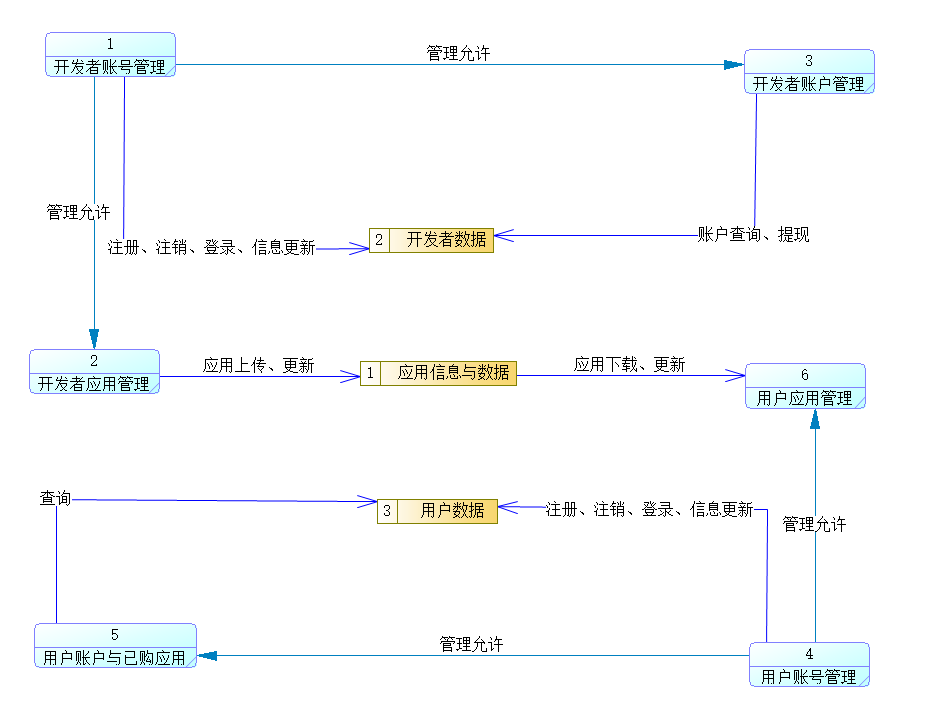
\includegraphics[width=12cm]{1_level_DFD_server.png}
	\caption{1层数据流图-服务器端} \label{fig:1_level_DFD_server}
\end{figure}

服务器的1层数据流图见图\ref{fig:1_level_DFD_server}

\section{数据字典}
\subsection{数据流说明}
\subsubsection{应用上载}

描述:开发者上传开发的应用

来源:开发者端

去处:服务器端(应用管理系统)

组成:应用ID+应用名+应用版本+应用描述+应用代码+开发者ID

\subsubsection{应用下载}

描述:用户下载应用

来源:服务器端(应用管理系统)

去处:客户端

组成:应用ID+应用名+应用版本+应用描述+可执行文件

\subsection{数据存储说明}
\subsubsection{应用}

流入数据流:添加、更新应用

流出数据流:检索、下载应用

组成:应用ID+应用名+应用版本+应用描述+应用代码+开发者ID+可执行文件

描述:应用的全部数据和信息

组织:按照特定类别排序

\subsubsection{用户信息}

流入数据流:用户注册、更新信息

流出数据流:用户登录

组成:用户ID+密码+基本信息+账户金额+已购买的应用

描述:用户的全部数据和信息

组织:按照用户ID排序

\subsubsection{开发者信息}

流入数据流:开发者注册、更新信息

流出数据流:开发者登录

组成:开发者ID+密码+基本信息+账户金额+开发的应用

描述:开发者的全部数据和信息

组织:按照开发者ID排序

\subsection{加工说明}
\subsubsection{应用检查}

\begin{lstlisting}[language=C, caption=示例代码, label={code:app_check}]
if(!secure_check(app)){
	return error.msg("not safe\n");
}
if(block_dev.has(app.info.dev)){
	return error.msg("blocked developer\n");
}
if(!running_test(app)){
	return error.msg("running error\n");
}
for(auto exist_app:app_list){
	if(similar_app(app,exist_app)>threshold){
		return error.msg("already exist app\n");
	}
}
app_list.push(app);

\end{lstlisting}

代码见\autoref{code:app_check} 

